\section{Espacio Geográfico}

% ── Frame: Contexto ───────────────────────────────────────────────────────────
% NOTA \pause: revela bullets uno a uno durante la presentación en vivo,
%   pero genera páginas PDF duplicadas. Descomenta solo si presentas en proyector.
\begin{frame}{CDMX: Un espacio complejo y diverso}
  \begin{columns}[T]
    \begin{column}{0.58\textwidth}
      \begin{itemize}
        \item La \zmvm\ es una de las urbes más antiguas del continente americano. Siendo fundada en 1325
        bajo el mandato del emperador Mexica Tenoch, con el nombre de Tenochtitlan (lugar de Tunas) \cite{molina2013erase}.
        % \pause
        \item  La ZMVM se constituye como una \termino{región nodal} donde la Ciudad de México actúa como centro articulador de 
                un sistema complejo de flujos, servicios y desigualdades socio-espaciales.
      \end{itemize}
    \end{column}
    \begin{column}{0.38\textwidth}
      \begin{block}{Dato clave}
        Los habitantes del \termino{cuarto contorno} metropolitano enfrentan tiempos de traslado que superan, en promedio, 
        los 122 minutos por viaje, resultado de una desconexión geométrica estructural que satura los nodos centrales \cite{tomtom2023traffic}.
      \end{block}
    \end{column}
  \end{columns}
\end{frame}


% ── Frame: Tres imágenes con texto explicativo ────────────────────────────────
\begin{frame}{Crecimiento Histórico}
  \begin{columns}[T]
    \begin{column}{0.5\textwidth}
      \begin{itemize}
        \item \textbf{1940-1980:} Fase de industrialización acelerada y crecimiento compacto.
        \item \textbf{1990-2010:} Transición hacia una \termino{urbanización difusa}, extendida y regional.
        \item En la CDMX, el área urbana se multiplicó \textbf{3.57 veces} entre 1970 y 2010, superando con creces el crecimiento demográfico \cite{padilla2022expansion}.
      \end{itemize}
    \end{column}
    \begin{column}{0.45\textwidth}
      \begin{figure}
        \centering
        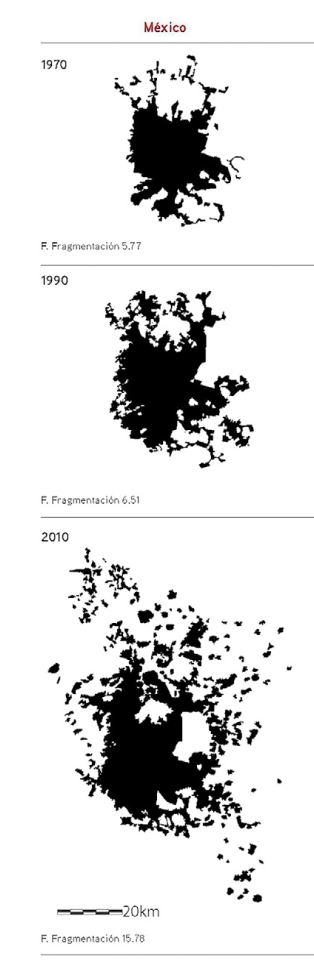
\includegraphics[width=\textwidth, height=5.5cm, keepaspectratio]{img/crecimiento_poblacional_fragmentacion_urbano_cdMexico.png}
        \caption{\textit{Evolución de la mancha urbana \cite{padilla2022expansion}.}}
      \end{figure}
    \end{column}
  \end{columns}
\end{frame}


% ── Frame: Tres imágenes con texto explicativo ────────────────────────────────
\begin{frame}{De la Ciudad a la Megalópolis: 1950 - 1970 - 2010}
  \begin{columns}[T]
    \begin{column}{0.32\textwidth}
      \centering
      \begin{alertblock}{\scriptsize Creación de los XII Cuarteles (1940)}
        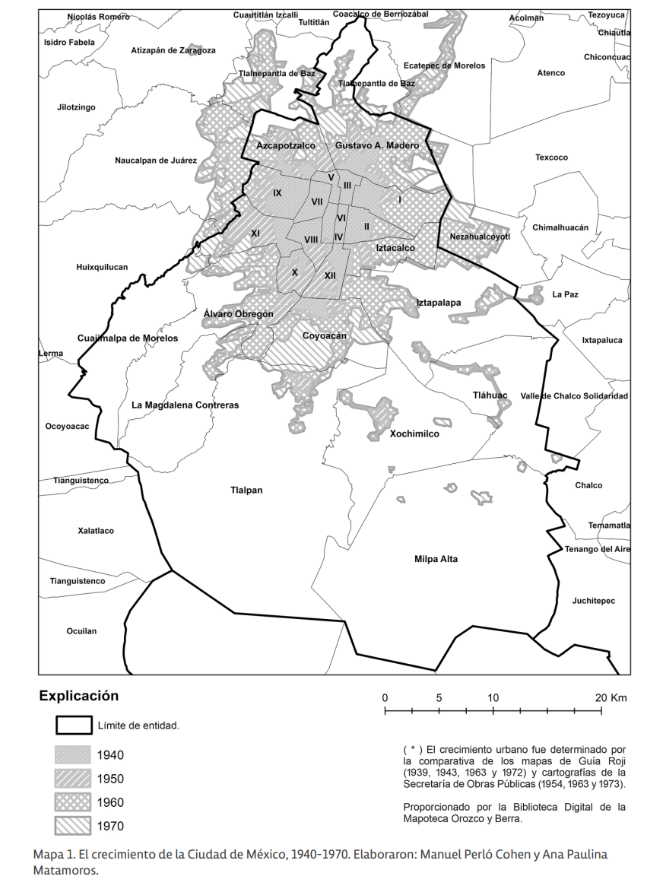
\includegraphics[width=\textwidth, height=3.5cm, keepaspectratio]{img/XII_Cuarteles.png}
        \scriptsize\texttt{
            \\
            En un inicio la Ciudad de México se planeo a través de XII Cuarteles.
            La vía de delimitación artificial fue el Anillo periférico.
        }
      \end{alertblock}
      {\scriptsize
      \fuentefigura{\cite{padilla2022expansion}}            
      .}\\[0.05cm]
    \end{column}

    \begin{column}{0.32\textwidth}
      \centering
      \begin{alertblock}{\scriptsize 1ra Expansión (1970)}
        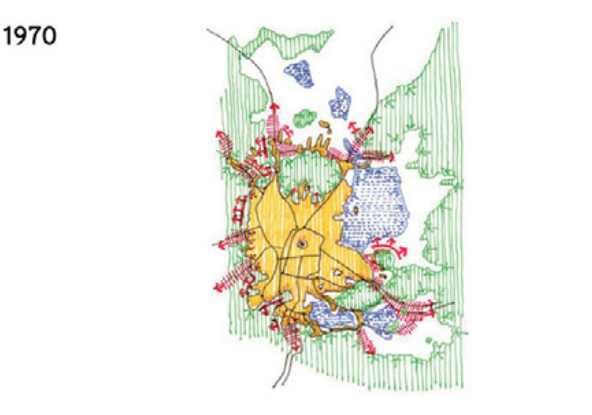
\includegraphics[width=\textwidth, height=3.5cm, keepaspectratio]{img/dispersion_cdMexico_1970.png}
        \scriptsize\texttt{
            \\
            Para 1970 en la CDMX, el área urbana se multiplicó \textbf{3.57 veces}.
        }
      \end{alertblock}
      {\scriptsize
      \fuentefigura{\cite{padilla2022expansion}}
      .}\\[0.05cm]
    \end{column}

    \begin{column}{0.32\textwidth}
      \centering
      \begin{alertblock}{\scriptsize 2da Expansión (20100)}
        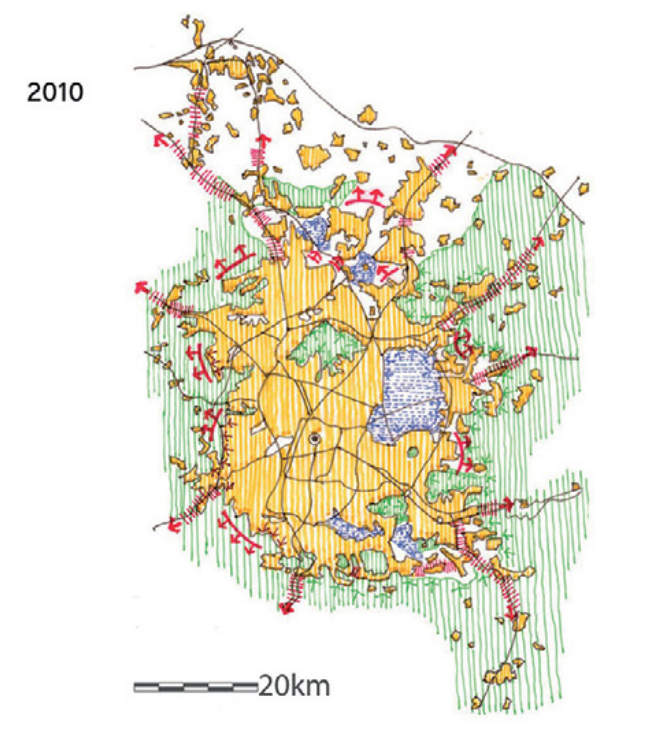
\includegraphics[width=\textwidth, height=3.5cm, keepaspectratio]{img/dispersion_cdMexico_2010.png}
        \scriptsize\texttt{
            \\
            Entre \textbf{1990-2010} hubo una transición hacia una \termino{urbanización difusa}, extendida y regional.
        }
      \end{alertblock}
      {\scriptsize
      \fuentefigura{\cite{padilla2022expansion}}
      .}\\[0.05cm]
    \end{column}
  \end{columns}
\end{frame}
